A central challenge in variational quantum machine learning is not merely to
build expressive quantum circuits, but to build the right expressive circuits.
Layered parameterized circuits with data re-uploading
~\cite{benedetti2019parameterized,perezsalinas2020data} can be highly flexible,
but flexibility alone is not a design principle. Without architectural
guidance, a model may spend parameters and data on distinctions irrelevant to
the task, while failing to allocate capacity to the structures that determine
the label. The practical question is therefore not only how much expressivity a
quantum model has, but where this expressivity is placed.

Symmetry is one of the few sources of prior knowledge that can be stated
exactly. Consider a target map \(y:\mathcal X \to \mathcal Y\) and a group
\(S\) acting on the input space through transformations
\(V_s:\mathcal X \to \mathcal X\). The task is invariant under \(S\) if
\[
    y(V_s[x]) = y(x)
    \qquad \text{for all } x \in \mathcal X,\; s \in S .
\]
In words, a symmetry specifies transformations of the input that must not
change the correct prediction. A translated image still depicts the same
object, a permuted graph still represents the same graph, and a rotated
Tic-Tac-Toe board still has the same winner. A model that respects this
structure by construction need not rediscover it from data.

This observation is central to geometric deep learning: classical
architectures such as convolutional neural networks organize trainable degrees
of freedom around task symmetries~\cite{cohen2016group}. In quantum machine
learning, geometric quantum machine learning represents known transformations
on the Hilbert space and constrains circuits accordingly
~\cite{larocca2022group,nguyen2024theory}. Related work has developed
group-invariant models, equivariant quantum neural networks,
permutation-equivariant architectures, graph-equivariant circuits, and
symmetry-informed variational ansatze
~\cite{larocca2022group,nguyen2024theory,skolik2023equivariant,sauvage2024building}.

\begin{figure*}[t]
\centering
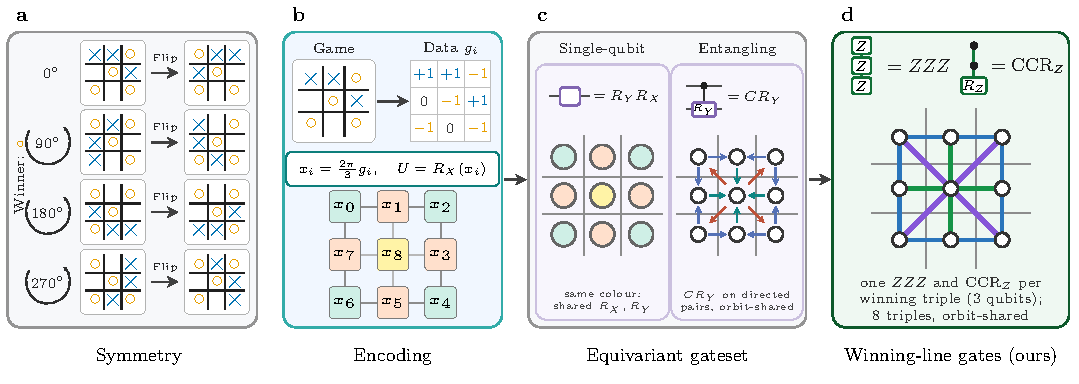
\includegraphics[width=0.98\textwidth]{fig1_4panel_standalone}
\caption{\normalsize From task symmetry to a task-aligned equivariant circuit.
(a) Tic-Tac-Toe labels are invariant under the $D_4$ rotations and reflections of the board.
(b) Board entries $g_i\in\{-1,0,+1\}$ are encoded as $R_X(x_i)$ rotations with $x_i=\frac{2\pi}{3}g_i$; the chosen indexing exposes the corner, side, and center orbits.
(c) The Meyer et al.~\cite{meyer2023symmetry} edge ansatz uses orbit-shared $R_YR_X$ rotations and directed $CR_Y$ entanglers on neighbouring and center-connected fields.
(d) Our extension adds orbit-shared $ZZZ$ and symmetric $CCR_Z$ gates on the eight winning triples, directly matching the label-relevant motifs while preserving equivariance.
Panel layout adapted from Meyer et al.~\cite{meyer2023symmetry}.}
\label{fig:protocol}
\end{figure*}

Meyer et al.~\cite{meyer2023symmetry} gave a concrete blueprint for this
program. If a data embedding \(U(x)\) satisfies
\[
    U(V_s[x]) = U_s U(x) U_s^\dagger ,
\]
then the data symmetry is represented by a unitary action \(U_s\). Trainable
blocks that commute with this representation, together with compatible state
preparation and readout, yield a model whose prediction is invariant by
architecture rather than by optimization.

However, symmetry alone does not specify an ansatz. It tells us which inputs
should be identified, which parameters may be shared, and which observables
should be aggregated, but not where trainable interactions should live. Two
circuits can respect the same group action and still match the task very
differently. We therefore treat symmetry not as a switch, but as a constrained
design space in which one must still choose the sharing strength and the motifs
on which trainable quantum interactions are placed.

Tic-Tac-Toe is a clean laboratory for this question. The task is finite,
exactly enumerable, and structurally transparent: each board has nine fields
and the label is determined by explicit three-cell winning lines. The relevant
symmetry is the dihedral group \(D_4\), containing the eight rotations and
reflections of the square. Acting on a \(3\times3\) board, \(D_4\) permutes the
nine fields while preserving the corner, side, and center orbits. Since these
transformations do not change whether crosses win, circles win, or the game is
a draw, the classification task is \(D_4\)-invariant.

Each board value \(g_i\in\{-1,0,+1\}\) is encoded on one qubit through a
Pauli-\(X\) rotation with angle \(x_i=2\pi g_i/3\). Under a board symmetry, the
encoded qubits are permuted like the board fields, so equivariance can be
imposed by sharing parameters across symmetry orbits of gates.

We separate two design choices that are usually entangled. The first is how
much symmetry to impose: full \(D_4\)-equivariance is natural, but smaller
subgroups may preserve most of the useful bias while leaving the circuit more
flexible. The second is where trainable interactions are placed. The
canonical \(D_4\)-equivariant Tic-Tac-Toe ansatz of Meyer et al. uses
orbit-shared single-qubit rotations and directed controlled rotations on
neighboring or center-connected fields~\cite{meyer2023symmetry}. This respects
the board symmetry, but the label is defined by complete rows, columns, and
diagonals. We therefore add task-aligned, orbit-shared \(ZZZ\) and symmetric
controlled-controlled-\(R_Z\) interactions on these winning triples.

Our numerical results support this design-oriented view. Enforcing board
symmetry improves generalization over an unshared edge ansatz, and suitable
subgroups recover much of the performance of full \(D_4\)-equivariance. The
largest improvement, however, comes from adding winning-line interactions to
the equivariant circuit. Thus, symmetry is not merely a constraint that makes a
model smaller. It is a language for organizing circuit design, but the
effectiveness of the model still depends on placing trainable degrees of
freedom where the structure of the task actually lives.
